\section{背景与理论框架}
\label{sec:background}

\subsection{传播、报告与两个估计目标}
\label{sec:bg-model}
\label{sec:meth-model}
\label{sec:meth-targets}

考虑第 $t$ 期的传播。上一代有 $n$ 名感染者，第 $i$ 人产生 $X_{i,t}$ 个继发感染。为刻画超传播，沿用 Lloyd-Smith 等\citep{lloydsmith2005superspreading}的设定，令给定 $R_t$ 时各 $X_{i,t}$ 相互独立并服从负二项分布
\begin{equation}
  X_{i,t}\mid R_t \sim \NB\!\left(k,\ \frac{k}{k+R_t}\right),\qquad
  \E(X_{i,t}\mid R_t)=R_t,\quad \Var(X_{i,t}\mid R_t)=R_t+\frac{R_t^2}{k},
  \label{eq:offspring}
\end{equation}
其中 $k$ 为离散参数，$k$ 越小，传播越集中于少数个体。式~\eqref{eq:offspring} 等价于个体再生数服从均值为 $R_t$、形状参数为 $k$ 的 Gamma 分布，继发感染数在其上服从泊松分布\citep{lloydsmith2005superspreading, endo2020estimating}。新感染总数 $I_t=\sum_{i=1}^{n}X_{i,t}$ 中，每人独立地以概率 $\rho$ 被报告，即 $C_t\mid I_t\sim\Bin(I_t,\rho)$。负二项分布取“失败次数”参数化时概率母函数为 $G(s)=p^{r}[1-(1-p)s]^{-r}$，独立和的母函数等于各项之积，二项稀疏对应 $G_C(s)=G_I(1-\rho+\rho s)$；代入 $p=k/(k+R_t)$ 可得
\begin{equation}
  G_C(s)=\frac{(p/q)^{nk}}{\{1-[(1-p)\rho/q]\,s\}^{nk}},\qquad q=1-(1-p)(1-\rho),
  \label{eq:thinning}
\end{equation}
即 $C_t$ 仍服从负二项分布：
\begin{equation}
  C_t\mid n,R_t \sim \NB\!\left(nk,\ \frac{k}{k+\rho R_t}\right),\qquad
  \E(C_t\mid n,R_t)=\rho nR_t,\quad
  \Var(C_t\mid n,R_t)=\rho nR_t+\frac{\rho^2nR_t^2}{k}.
  \label{eq:report-dist}
\end{equation}
记 $m=\rho n$ 为上一代感染者中预计被报告的人数，下文称为预计报告规模，并用它度量监测规模。报告数的相对方差由报告抽样与超传播两部分组成：
\begin{equation}
  \frac{\Var(C_t\mid n,R_t)}{\E(C_t\mid n,R_t)^2}=\frac{1}{\rho nR_t}+\frac{1}{nk}.
  \label{eq:relvar}
\end{equation}
提高报告率 $\rho$ 可以压低第一项；第二项只能靠增加感染者人数 $n$ 压低。

$R_t$ 随时间波动。天气、学校假期和人群流动使各期传播强度围绕平均水平变化\citep{dalziel2018urbanization, rasmussen2011inference}，记 $\E(R_t)=\Rbar$，$\Var(R_t)=v_R$，称 $v_R$ 为环境方差。生态学把同一期内全体个体共享的波动称为环境随机性，以区别于个体层面的人口随机性\citep{engen1998demographic, rohani2002determinism}。监测问题据此分为两个估计目标。估计目标1是条件估计目标，即给定当期环境时实际发生的瞬时再生数 $R_t$，例如判断本周传播是否快于上周。估计目标2是边缘估计目标，即各期再生数所围绕的跨期平均再生数 $\Rbar$。各期环境独立时，后者也是下一期传播水平的一步前瞻预测；以此前 $T_0$ 期估计 $\Rbar$ 时，预测误差乘以 $1+1/T_0$。两个目标共用估计量 $\widehat R_t=C_t/m$，区别在于误差的参照对象：估计目标1的误差为 $\widehat R_t-R_t$，估计目标2的误差为 $\widehat R_t-\Rbar$，后者多出一项不随规模变化的 $R_t-\Rbar$。Eales 与 Riley（\citeyear{eales2024differences}）讨论的表观再生数，是由一条病例序列和给定世代间隔反推的加权平均，它滞后并平滑真实再生数；本文的估计目标1对应条件瞬时值，估计目标2对应跨期均值，二者都不是表观再生数本身，但在使用滞后计数构造增长统计量时会受到类似的卷积影响（第~\ref{sec:meth-renewal}~节）。

上述推导依赖以下四条假设。
\begin{enumerate}[label=H\arabic*]
  \item 给定 $R_t$，各感染者的继发感染数相互独立且服从式~\eqref{eq:offspring}，报告过程为独立二项抽样。
  \item 同一期的感染者共享同一个 $R_t$，环境扰动作用在期的层面。
  \item 离散参数 $k$ 与报告率 $\rho$ 已知。
  \item 规模 $n$ 与当期环境无关，即 $\E(R_t\mid n)=\Rbar$，$\Var(R_t\mid n)=v_R$；作一步预测时，还要求 $R_{t+1}$ 与截至第 $t$ 期的全部信息独立。
\end{enumerate}
若 $n$ 由设计固定，例如每期追踪固定数目的指示病例，H4 自然成立。若 $n_t$ 是此前传播的结果，而 $R_t$ 又有时间相关，较大的 $n_t$ 往往出现在 $R_t$ 偏高的时期，H4 不再自动成立。真实监测序列属于后一种情况，第~\ref{sec:meth-renewal}~节的更新过程设定与第~\ref{sec:meth-sim}~节的一阶自回归仿真专门处理它。H3 在实践中也只是近似，$k$ 需要估计。

\begin{figure}[!p]
  \centering
  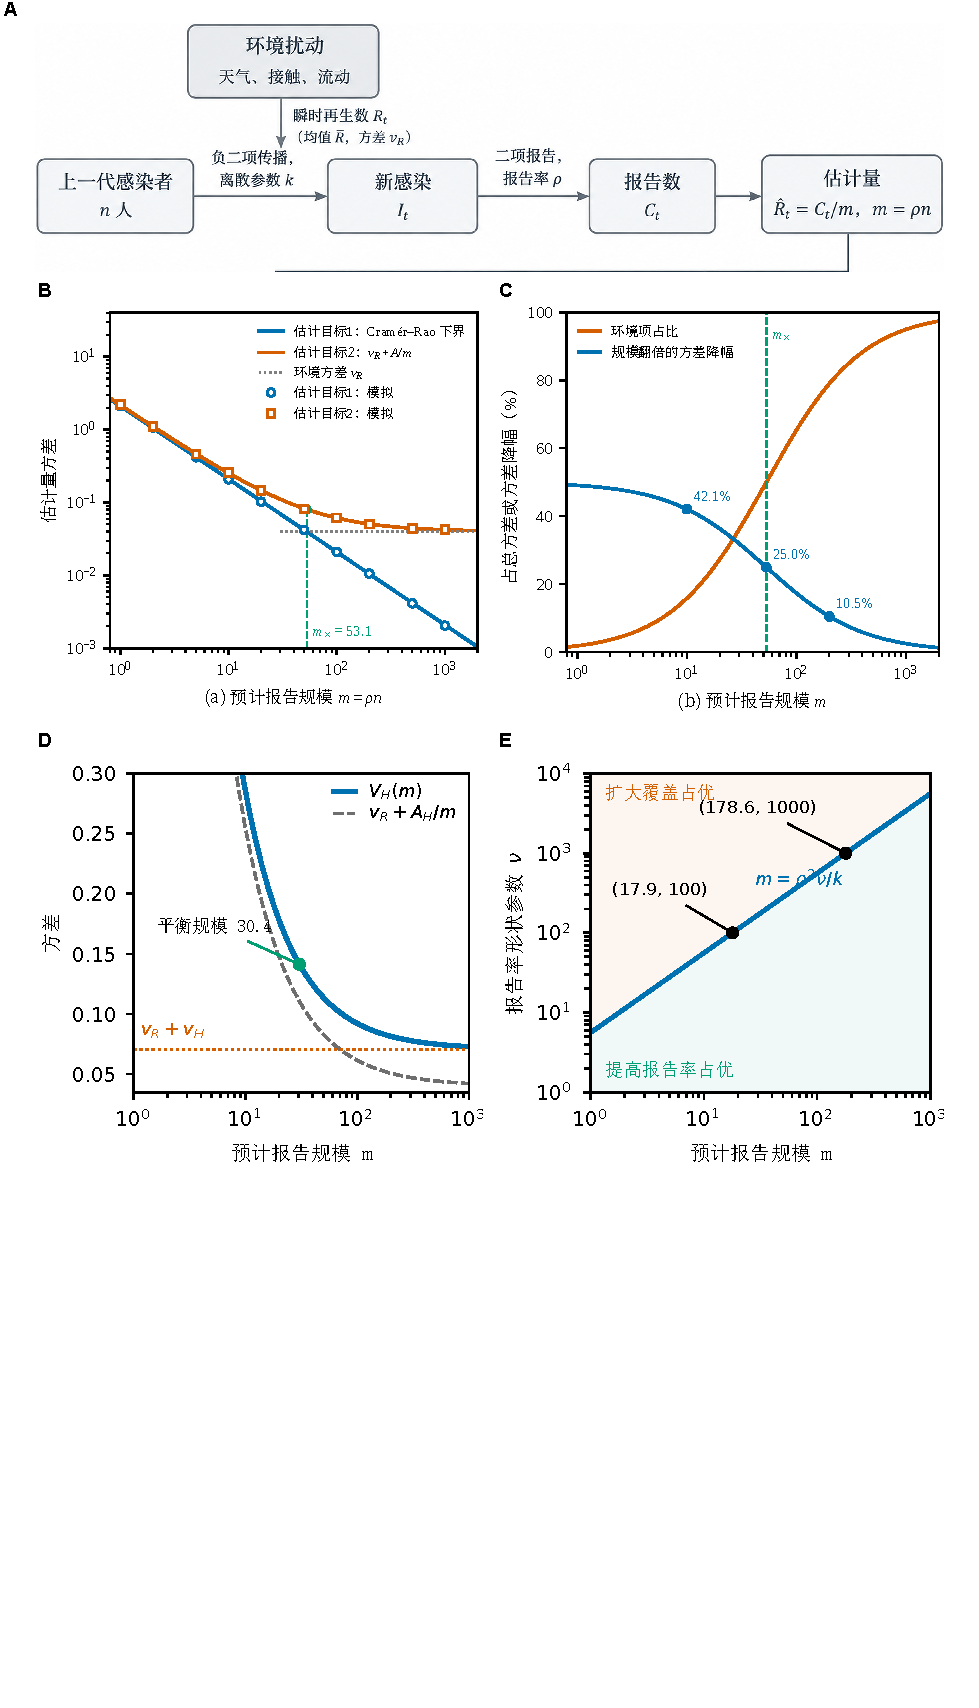
\includegraphics[width=0.98\textwidth]{figures/fig_main1.pdf}
  \caption{模型与方差结构。(A) 传播与报告过程：环境扰动决定当期瞬时再生数 $R_t$，上一代 $n$ 名感染者按负二项分布产生新感染 $I_t$，新感染经二项报告成为报告数 $C_t$，由此得到估计量 $\widehat R_t=C_t/m$；下排为同一估计量对应的两个估计目标。(B) 两个估计目标的方差随预计报告规模 $m$ 的变化，参数为 $\Rbar=1.15$、$v_R=0.04$、$k=0.35$、$\rho=0.25$，对应 $A=2.1232$、$\mx=53.1$；空心点为每个规模 20{,}000 次模拟的方差，绿色虚线标出方差平衡规模。(C) 环境项在总方差中的占比与规模翻倍带来的方差降幅随 $m$ 的变化，点线标出 $m=10$、$\mx=53.1$、$m=200$ 处的降幅 42.1\%、25.0\% 和 10.5\%。(D) 报告率逐期波动时式~\eqref{eq:r3-vH} 的方差曲线，$\tau=0.15$，方差平衡规模由 53.1 降到 30.4，点线为 $v_R+v_H$。(E) 二项型报告波动下提高报告率与扩大覆盖的排序反转边界，曲线两侧分别对应提高报告率占优与扩大覆盖占优。}
  \label{fig:variance}
\end{figure}

\subsection{方差分解与平衡规模}
\label{sec:bg-variance}

瞬时再生数能被测到多准，由单期报告数关于 $R_t$ 的 Fisher 信息决定。对估计目标1，$R_t$ 视为固定参数，估计量的性质由式~\eqref{eq:report-dist} 直接给出。

\begin{proposition}[瞬时再生数的有效估计]
\label{prop:current}
在 H1--H3 下，给定 $n$ 与 $R_t>0$，估计量 $\widehat R_t=C_t/m$ 是 $R_t$ 的极大似然估计，无偏，方差为
\begin{equation}
  \Var(\widehat R_t\mid n,R_t)=\frac{R_t}{\rho n}+\frac{R_t^2}{kn},
  \label{eq:var-current}
\end{equation}
并在每个有限 $n$ 处等于 Cramér--Rao 下界 $1/\mathcal I(R_t)$，其中 $\mathcal I(R_t)=n/(R_t/\rho+R_t^2/k)$。$C_t=0$ 时似然在边界 $R_t=0$ 处取最大值。$k$ 已知时，$\widehat R_t$ 还是 $R_t$ 的一致最小方差无偏估计。
\end{proposition}

式~\eqref{eq:var-current} 的两部分与式~\eqref{eq:relvar} 的两项一一对应：$R_t/(\rho n)$ 来自报告抽样，$R_t^2/(kn)$ 来自超传播，二者都按 $1/n$ 衰减。Fisher 信息可改写为 $\mathcal I(R_t)=(m/R_t)(1+\rho R_t/k)^{-1}$，$k\to\infty$ 时趋于 $m/R_t$，与 Parag 等\citep{parag2022quantifying}在泊松更新模型下给出的发病曲线信息一致。超传播使每个预计报告病例所含的信息按因子 $(1+\rho R_t/k)^{-1}$ 缩减。蒙特卡洛模拟在 $m$ 从 1 到 1000 的 10 个规模上各重复 20{,}000 次，模拟方差与下界之比为 0.98--1.02。只要监测关心的是当期传播强度，扩大规模的收益就不会饱和。

监测目标换成 $\Rbar$ 以后，误差中有一部分不再随规模下降，其大小由环境方差决定。

\begin{proposition}[跨期平均再生数的估计方差]
\label{prop:average}
在 H1--H4 下，$\widehat R_t=C_t/m$ 是 $\Rbar$ 的无偏估计，其方差为
\begin{equation}
  V(m)=\Var(\widehat R_t\mid n)=v_R+\frac{\Rbar}{\rho n}+\frac{\Rbar^2+v_R}{kn}
  =v_R+\frac{A}{m},\qquad A=\Rbar+\frac{\rho(\Rbar^2+v_R)}{k}.
  \label{eq:var-average}
\end{equation}
定义方差平衡规模 $\mx=A/v_R$。该规模仅表示抽样项与环境项相等的方差平衡点，并非满足特定估计精度或预警功效要求的最低监测规模。当 $m\to\infty$ 时 $V(m)\to v_R$；规模项在总方差中占 $1/(1+m/\mx)$，在 $m=\mx$ 处两项各半；规模从 $m$ 翻倍到 $2m$ 时方差下降 $1/[2(1+m/\mx)]$；$V(m)$ 严格递减且严格凸，弹性为 $-\mx/(m+\mx)$，在 $m=\mx$ 处等于 $-1/2$。在对 $R_t$ 条件无偏的估计类中，$V(m)$ 是 $\Rbar$ 的最小均方误差；在 H4 下也是以过去数据预测下一期增长 $C_{t+1}/m$ 的最小预测均方误差。
\end{proposition}

式~\eqref{eq:var-average} 由全方差公式得到，条件方差的期望给出 $A/m$，条件均值 $R_t$ 的方差给出 $v_R$。比较命题~\ref{prop:current} 可知 $A/m=\E[1/\mathcal I(R_t)]$，估计目标2的方差等于环境方差加上估计目标1的 Cramér--Rao 下界在环境分布上的平均。对任一在给定 $R_t$ 时无偏的估计量 $\tilde\theta$，把误差拆为 $(\tilde\theta-R_t)+(R_t-\Rbar)$，交叉项的期望为零，由全方差公式得
\begin{equation}
  \E(\tilde\theta-\Rbar)^2=\E\big[\Var(\tilde\theta\mid R_t)\big]+v_R
  \ \geq\ v_R+\E\big[1/\mathcal I(R_t)\big]=v_R+\frac{A}{m},
  \label{eq:unbiased-bound}
\end{equation}
其中第二个等号用到 $\E(R_t^2)=\Rbar^2+v_R$。$\widehat R_t=C_t/m$ 取到等号，故 $V(m)$ 是该估计类的最小均方误差。在 H4 下，若下一期规模 $m$ 已知，任何以截至第 $t$ 期的信息为依据的预测量 $\hat y$ 对 $y=C_{t+1}/m$ 的误差满足
\begin{equation}
  \E(\hat y-y)^2\ \geq\ \Var(y\mid\mathcal F_t)=v_R+\frac{A}{m},
  \label{eq:predict-bound}
\end{equation}
等号由 $\hat y=\Rbar$ 取到。这一下界不要求无偏性，但依赖各期环境独立；$\Rbar$ 未知而用此前 $T_0$ 期估计时，误差乘以 $1+1/T_0$。

$V(m)$ 处处凸，曲线上没有拐点，方差平衡规模给出的是一个量纲为病例数的比较基准：规模低于 $\mx$ 时误差主要来自病例数不足，高于 $\mx$ 时误差主要来自环境波动，翻倍带来的方差降幅很快变小。图~\ref{fig:variance}B 取 $\Rbar=1.15$、$v_R=0.04$、$k=0.35$、$\rho=0.25$，对应 $A=2.1232$、$\mx=53.1$；规模为 10、53.1 和 200 时，翻倍带来的方差降幅依次为 42.1\%、25.0\% 和 10.5\%。

环境方差下确界的适用范围由命题~\ref{prop:average} 的最后一条限定，即单期、对 $R_t$ 条件无偏的估计，以及 $\phi=0$ 时的一步前瞻预测。$R_t$ 服从系数为 $\phi$ 的一阶自回归时，借用前期信息作预测，不可约的环境部分为 $(1-\phi^2)v_R$，$\phi=0.5$ 与 $0.8$ 时分别为 $0.75v_R$ 与 $0.36v_R$。汇总多个辖区同样可以压低环境项。设 $J$ 个辖区的环境方差同为 $v_R$，两两相关系数的平均值为 $\bar c$，等权汇总后的环境项为
\begin{equation}
  v_R\,\bar c+\frac{v_R(1-\bar c)}{J}.
  \label{eq:pooling}
\end{equation}
各辖区的扰动不完全同步时（$\bar c<1$），汇总能降低环境项；完全同步时汇总无效。

\begin{remark}[报告率与覆盖面]
\label{rem:reporting}
预计报告规模 $m=\rho n$ 可以靠提高报告率 $\rho$ 或扩大覆盖人群 $n$ 增大。固定 $n$ 令 $\rho\to1$ 时，$V\to v_R+\Rbar/n+(\Rbar^2+v_R)/(kn)$，极限严格大于 $v_R$；固定 $\rho$ 令 $n\to\infty$ 时 $V\to v_R$。把 $n$ 与 $\rho$ 各提高相同的小比例，前者带来的方差下降是后者的 $A/\Rbar=1+\rho(\Rbar^2+v_R)/(k\Rbar)$ 倍。
\end{remark}

报告完全时超传播项依然存在，只有扩大覆盖才能把方差压到 $v_R$。在图~\ref{fig:variance} 的参数下 $A/\Rbar=1.85$；流感住院占感染的比例约为 0.6\%--2\%\citep{zhou2012hospitalizations, tokars2018seasonal}，在第~\ref{sec:res-case}~节的情景参数下该倍数只有 1.02--1.18，两条途径的效果几乎相同，选择主要取决于成本。注~\ref{rem:reporting} 假设报告率在各期固定，报告率随期波动时见第~\ref{sec:bg-reporting}~节。

\subsection{报告异质性与可识别性}
\label{sec:bg-reporting}

报告比例逐期波动时，不可约误差中多出一个与规模无关的分量。H1 把报告视为固定概率 $\rho$ 的二项抽样，这里用以下两条假设替代其中的报告部分。
\begin{enumerate}[label=H\arabic*,start=5]
  \item 第 $t$ 期的报告率 $p_t\in(0,1]$ 随机，给定 $p_t$ 时每例新感染独立地以概率 $p_t$ 被报告；$\{p_t\}$ 平稳，与 $\{R_t\}$ 及 $n$ 独立，$\E p_t=\rho$，$\Var p_t=\sigma^2$。记相对波动 $\tau=\sigma/\rho$ 与标准化报告率 $u_t=p_t/\rho$。
  \item 给定 $(R_1,\dots,R_T)$ 与 $(p_1,\dots,p_T)$，各期报告数相互独立。
\end{enumerate}
把式~\eqref{eq:thinning} 推导中的 $\rho$ 换成 $p_t$，即得 $C_t\mid n,R_t,p_t\sim\NB(nk,\,k/(k+p_tR_t))$。二项型波动来自报告率本身的抽样，例如 $p_t\sim\mathrm{Beta}(\rho\nu,(1-\rho)\nu)$，此时 $\sigma^2=\rho(1-\rho)/(\nu+1)$，$\rho\to1$ 时波动消失；制度型波动来自填报口径或检测政策的变化，相对波动 $\tau$ 与 $\rho$ 无关。

\begin{proposition}[报告率波动下的方差三分量]
\label{prop:report-noise}
在 H1--H5 下，记 $U=(1+\tau^2)(\Rbar^2+v_R)$。给定 $(n,R_t)$ 时，条件方差为
\begin{equation}
  \Var(C_t\mid n,R_t)=\rho nR_t+\frac{(\rho^2+\sigma^2)nR_t^2}{k}+\sigma^2n^2R_t^2,
  \label{eq:r3-var-cond}
\end{equation}
$\widehat R_t=C_t/m$ 仍是 $\Rbar$ 的无偏估计，方差分为三项：
\begin{equation}
  V_H(m)=v_R+v_H+\frac{A_H}{m},\qquad
  v_H=\tau^2(\Rbar^2+v_R),\qquad
  A_H=\Rbar+\frac{\rho(1+\tau^2)(\Rbar^2+v_R)}{k}.
  \label{eq:r3-vH}
\end{equation}
$v_H$ 与覆盖人数 $n$ 无关，推广的方差平衡规模为 $m_{\times,H}=A_H/(v_R+v_H)$。记 $\mathcal J_u=\E\{[1+u_tf_u'(u_t)/f_u(u_t)]^2\}$，$f_u$ 为 $u_t$ 的密度，则对任一只用 $C_t$ 且对 $R_t$ 条件无偏的估计量 $\tilde\theta$ 与任一规模 $m$，
\begin{equation}
  \E(\tilde\theta-\Rbar)^2\ \geq\ v_R+\frac{\Rbar^2+v_R}{\mathcal J_u},\qquad \mathcal J_u\geq\frac{1}{\tau^2},
  \label{eq:r3-lb}
\end{equation}
后一不等式当且仅当 $u_t$ 服从 Gamma 分布时取等号。若各期 $p_t$ 可观测且 $\E(1/p_t)<\infty$，估计量 $\tilde R_t=C_t/(p_tn)$ 对 $R_t$ 条件无偏，均方误差为
\begin{equation}
  \E(\tilde R_t-\Rbar)^2=v_R+\frac{\Rbar\,\E(1/p_t)}{n}+\frac{\Rbar^2+v_R}{kn},
  \label{eq:r3-obs}
\end{equation}
其中不含 $v_H$，$n\to\infty$ 时趋于 $v_R$。仅用报告数的前两阶矩时，$(v_R,\tau^2)$ 只通过 $U$ 进入均值和方差：$v_R+v_H=U-\Rbar^2$，$A_H=\Rbar+\rho U/k$，二者不可分。设第 $j$ 个辖区的报告率为 $p_{j,t}=\rho_ju_{j,t}$，$\rho_j$ 不随时间变化，$u_{j,t}$ 平稳，$\Var u_{j,t}=\tau_w^2$，自相关为 $\psi^h$。增长统计量 $G_t=C_{t+1}/D_t$ 中 $\rho_j$ 精确约去。记 $G_t^0$ 为报告率恒为 $\rho_j$ 时的增长统计量；在无计数噪声、滞后窗口内真实感染数近似不变时，$\E(G_t/G_t^0-1)^2=\tau_w^2F(w,\psi)+o(\tau_w^2)$，其中
\begin{equation}
  F(w,\psi)=1-2\sum_{s\geq1}w_s\psi^{s}+\sum_{s\geq1}\sum_{s'\geq1}w_sw_{s'}\psi^{|s-s'|}.
  \label{eq:r3-F}
\end{equation}
\end{proposition}

命题~\ref{prop:report-noise} 的前两条把命题~\ref{prop:average} 的两项扩展为 $v_R+v_H+A_H/m$：$v_H$ 与环境方差一样不随规模下降，$A_H$ 中的 $(1+\tau^2)$ 使规模项同时放大。$v_H$ 中没有超传播带来的 $1/k$ 因子，原因是超传播项随 $n$ 下降，而报告率波动作用在整期报告数上。第三条用数据处理不等式给出规模无法消除的部分：$C_t$ 只经过 $p_tR_t$ 依赖 $R_t$，其 Fisher 信息不超过与 $m$ 无关的 $\mathcal J_u/R_t^2$；$u_t$ 服从 Gamma 分布时下界与规模无关且等于 $v_R+v_H$，$\widehat R_t$ 在 $m\to\infty$ 时趋于该下界，$v_R+v_H$ 因此是这一估计类在全部规模上的下确界。第四条说明报告率可观测时，把计数除以 $p_t$ 可以去掉 $v_H$。第五条说明只看均值和方差无法把环境波动与报告波动分开：沿 $U$ 的等值线改变 $(v_R,\tau^2)$，报告数的前两阶矩不变。第六条给出一个可以用数据检验的签名：报告噪声使预测误差的截距按 $F(w,\psi)$ 随滞后权重变化，而平稳环境方差使截距与权重无关。

\begin{corollary}[覆盖与报告率排序的反转阈值]
\label{cor:switch}
在命题~\ref{prop:report-noise} 的条件下，把 $\rho$ 或 $n$ 各提高相同的小比例，提高报告率带来的方差下降大于扩大覆盖，当且仅当
\begin{equation}
  -\rho\,\frac{\mathrm d\tau^2}{\mathrm d\rho}\,(kn+1)\ >\ 1+\tau^2 .
  \label{eq:r3-switch}
\end{equation}
二项型波动下，该条件等价于 $m>\rho^2\nu/k$，规模足够大时提高报告率占优；$\nu\to\infty$ 时 $\sigma^2\to0$，条件不再成立。制度型波动下，覆盖与报告率的边际效果之比为 $A_H/\Rbar>1$，覆盖始终占优，两条途径都不改变 $v_H$。
\end{corollary}

推论~\ref{cor:switch} 限定了固定报告率下的排序。二项型波动下，提高报告率还能压低报告率本身的波动，$\rho=0.25$、$k=0.35$、$\nu=100$ 时排序在 $m>17.9$ 处反转，$\nu=1000$ 时在 $m>178.6$ 处反转。制度型波动下，图示参数与 $\tau=0.15$ 给出的边际效果之比为 1.87，与固定报告率时的 1.85 接近，两条途径都留下 $v_H$。去掉 $v_H$ 需要统一报告口径使 $\tau\to0$，或像命题~\ref{prop:report-noise} 第四条那样把各期报告率纳入估计。

图示参数下取 $\tau=0.15$，$v_H=0.0307$，$A_H=2.145$，推广的方差平衡规模由 53.1 降到 30.4；$m=1000$ 时 $V_H=0.0728$，而 $v_R+A/m=0.0421$（图~\ref{fig:variance}D）。纯报告噪声对截距比的预测为 $q_1\in[0.883,1.338]$、$q_2\in[0.892,1.374]$（$\psi\in[0,1)$）；这个范围是后文判断报告签名是否成立的基准。二项型波动下 $\E(1/p_t)=(\nu-1)/(\rho\nu-1)$，要求 $\rho\nu>1$；$\rho=0.25$、$\nu=100$ 时为 4.125。制度型波动取 $u_t$ 服从形状与速率同为 $1/\tau^2$ 的 Gamma 分布时，$\E(1/u_t)=1/(1-\tau^2)$，要求 $\tau<1$。这些条件说明式~\eqref{eq:r3-obs} 的可积性并非自动成立，报告率接近零的时期会使均方误差发散。
